\documentclass[11pt,twocolumn]{article}
\usepackage[margin=0.72in]{geometry}
\usepackage{amsmath,amssymb,amsthm}
\usepackage{booktabs}
\usepackage{graphicx}
\usepackage{hyperref}
\usepackage{xcolor}
\usepackage{enumitem}

\hypersetup{
  colorlinks=true,
  linkcolor=blue!60!black,
  citecolor=green!45!black,
  urlcolor=blue!65!black
}

\newtheorem{proposition}{Proposition}
\newtheorem{definition}{Definition}

\newcommand{\ZZ}{\mathbb{Z}}
\newcommand{\NN}{\mathbb{N}}

\title{\textbf{Machine-Checked Exact-Integer Simultaneous Tiling, Hole-Move Repair, and Laurent Divisibility-Boosting Certificates for Dominoes Tiling a Common Figure}}
\author{Lluis Eriksson\thanks{Independent researcher; manuscript prepared with transparent AI assistance via Google Antigravity. Source code, Lean~4 proofs, and exact certificates: \url{https://github.com/lluiseriksson/dominoes-common-figure-certificates}.}}
\date{November 25, 2026}

\begin{document}
\maketitle

\begin{abstract}
Peter Keevash and Jeck Lim (\texttt{arXiv:2611.33154}, November 24, 2026) resolved Sagdeev's problem affirmatively (Theorem~1.2): for any finite collection of arithmetic progressions (in particular, dominoes) $D_1,\dots,D_k \subset \ZZ^2$, there exists a finite non-empty lattice figure $B \subset \ZZ^2$ that can be partitioned into disjoint translates of every~$D_i$. Their proof reduces all $D_i$ to primitive directions and a common length~$d$, relaxes $\{0,1\}$-tileability to integral Laurent-polynomial \emph{tile divisibility} in $\ZZ[x_1^{\pm 1}, x_2^{\pm 1}]$ (Step~5, via unimodular basis-change divisibility boosting), and repairs tile-divisible lines into genuinely tileable lines via step-$d$ hole moves (Step~6). We present a machine-checked, zero-floating-point formalization and exact-$\ZZ$ certificate auditor for the finite combinatorial, algebraic, and repair core of this work. First, an 18-theorem zero-dependency Lean~4 kernel (\texttt{DominoesCommonFigure.lean}, Lean~4.35.0; 0~\texttt{sorry}, 0~warnings, 0~\texttt{Classical.choice}, 2 zero-axiom theorems) formalizes primitive-stretch and common-length LCM partitions, $(1-t)D_d(t) = 1-t^d$, explicit $d=2$ and $d=3$ tile-divisible-yet-untileable gap witnesses ($1+t^2+t^3+t^5$ and $1+t^2+t^4$), exact single step-$d$ hole-move repairs, unimodular $\det=1$ Cramer basis decomposition, Laurent divisibility boosting, and parallel-line conservation. Second, \texttt{DOMINO-AP-TILING-CERT-1.0} audits four exact modes—including a $D_4$-symmetric 48-cell 4-direction Sagdeev queen-domino figure tiled simultaneously by 24 dominoes in each of $(1,0),(0,1),(1,1),(1,-1)$—replaying 16 canonical certificates in $0.030$--$0.292\,\mathrm{ms}$, quantifying the growing Step~5--6 gap ($64.9\%$ for $d=2, L=10$; $82.9\%$ for $d=3, L=12$), and rejecting 61/61 live adversarial forgeries.
\end{abstract}

\section{Introduction}
A two-element subset $D = \{0, v\} \subset \ZZ^2$ is a \emph{domino}, and more generally $D = \{0, v, \dots, (d-1)v\}$ ($d \ge 2$) is an \emph{arithmetic progression (AP)}. Sagdeev~\cite{sagdeev2024mathoverflow} asked whether every finite family of dominoes $D_1,\dots,D_k \subset \ZZ^2$ tiles a common finite non-empty figure $B \subset \ZZ^2$, noting simple solutions for standard dominoes ($2\times 2$ square) and queen dominoes, while adding a single gap domino $D_5 = \{(0,0),(2,0)\}$ already required a SAT-discovered 416-cell figure. Keevash and Lim~\cite{keevash2026dominoes} proved the full general theorem for arbitrary APs (Theorem~1.2), coupling the polynomial-decomposition machinery of their companion paper~\cite{keevash2026reconfig} with a six-step algebraic hypergraph absorption scheme extending classical Conway--Lagarias tiling algebra~\cite{conway1990tiling}.

Three finite algebraic mechanisms drive~\cite{keevash2026dominoes}: (i)~preprocessing arbitrary APs to primitive directions ($v = c v' \mapsto$ length $cd$) and a common length $L = \mathrm{lcm}(c_i d_i)$ (Section~2); (ii)~boosting integral Laurent divisibility in $\ZZ[X_1^{\pm 1}, X_2^{\pm 1}]$ via unimodular basis changes $\det(X_1, X_2) = 1$ and modulo-$(X_1^d - 1)$ polynomial lifting (Step~5, Section~2.1); and (iii)~bridging the strict gap between signed integral divisibility ($Q \in \ZZ[t]$) and true $\{0,1\}$-tileability ($Q \in \ZZ_{\ge 0}[t]$) via step-$d$ hole moves (Step~6).

\paragraph{Contributions.}
We formally verify and audit the finite tiling, preprocessing, gap-repair, and Laurent divisibility-boosting core of~\cite{keevash2026dominoes} (explicitly scoping our Lean~4 proofs away from the Markov-chain jagged boundary construction, almost-perfect matching hypergraph nibble, and asymptotic $O(n^{1-\delta})$ absorption constants of Steps~1--4):
\begin{enumerate}[leftmargin=*,nosep]
  \item \textbf{Zero-dependency Lean~4 kernel (\S\ref{sec:lean}):} 18 constructive theorems in \texttt{DominoesCommonFigure.lean} (Lean~4.35.0~\cite{demoura2021lean4}), 0~\texttt{sorry}, 0~warnings, 0~\texttt{Classical.choice}, 2 zero-axiom theorems.
  \item \textbf{Exact-$\ZZ$ tiling \& boosting verifier (\S\ref{sec:certifier}):} \texttt{DOMINO-AP-TILING-CERT-1.0}, auditing simultaneous AP tilings, Step~5--6 gap/hole-move repairs, Section~2.1 unimodular Laurent divisibility lifts, and primitive/LCM reductions with zero floats.
  \item \textbf{48-cell Sagdeev figure, gap census, \& red-team audit (\S\ref{sec:results}):} 16 canonical certificates (including a $D_4$-symmetric 48-cell 4-direction Sagdeev figure) replayed in $0.030$--$0.292\,\mathrm{ms}$, exhaustive 1D gap censuses, and 61/61 rejected adversarial forgeries.
\end{enumerate}

\section{Algebraic Structure of Common-Figure Tilings}\label{sec:prelim}
Identify a finite set $B \subset \ZZ^2$ with $P_B(x_1, x_2) = \sum_{(a_1,a_2)\in B} x_1^{a_1} x_2^{a_2} \in \ZZ[x_1^{\pm 1}, x_2^{\pm 1}]$ and an AP $D = \{0, v, \dots, (d-1)v\}$ with $P_D(x) = \sum_{j=0}^{d-1} x^{jv}$. A disjoint-translate tiling of $B$ by $D$ is equivalent to $P_B = P_D \cdot Q$ with $Q \in \{0,1\}[x_1^{\pm 1}, x_2^{\pm 1}]$, whereas \emph{tile divisibility} (Step~5) relaxes $Q$ to $\ZZ[x_1^{\pm 1}, x_2^{\pm 1}]$. Along a 1D line, even simple sets exhibit a strict gap:
\begin{equation}
\begin{aligned}
  1 + t^2 + t^3 + t^5 &= (1 + t)(1 - t + 2t^2 - t^3 + t^4), \\
  1 + t^2 + t^4 &= (1 + t + t^2)(1 - t + t^2),
\end{aligned}
  \label{eq:gap}
\end{equation}
both divisible in $\ZZ[t]$ yet untileable (since $q_0 = 1$ forces $q_0 + q_1 \ge 1 \neq 0$ for any $q_0, q_1 \in \NN$). Moving a single hole by a multiple of~$d$ ($1 \mapsto 5$ for $d=2$; $1 \mapsto 4$ for $d=3$) preserves $h \bmod d$ while eliminating every negative coefficient of~$Q$.

In Step~5 divisibility boosting (Section~2.1), choosing a unimodular basis $(X_1, X_2)$ with $X_1 = v_i$, $\det(X_1, X_2) = 1$, and $v_j = u_1^{(j)} X_1 + u_2^{(j)} X_2$ ($j < i$), any $f$ divisible by $X^{d u^{(j)}} - 1$ ($j < i$) with $X_1^d - 1 \mid (f - F^*)$ is boosted by lifting $\pi(F^*) \bmod (X_1^d - 1)$ to $F$ satisfying
\begin{equation}
\begin{aligned}
  (X_1^d - 1) &\mid (f - F), \\
  (X^{d u^{(j)}} - 1) &\mid (f - F)\quad (\forall j < i).
\end{aligned}
  \label{eq:boost}
\end{equation}

\section{Zero-Dependency Lean 4 Kernel}\label{sec:lean}
We formalize 18 constructive theorems in \texttt{lean/DominoesCommonFigure.lean} (Lean~4.35.0, zero external libraries), audited via \texttt{lean/AuditAxioms.lean} with 0~warnings, 0~\texttt{sorry}, 0~\texttt{Classical.choice}, and 0~\texttt{Lean.ofReduceBool} (Table~\ref{tab:lean}).

\begin{proposition}[Constructive Domino \& Boosting Kernel]\label{prop:lean}
\leavevmode
\begin{enumerate}[leftmargin=*,nosep]
  \item \emph{Tiling \& preprocessing partitions:} Theorems~1--4 and~16--18 prove $d \mid |B|$, $2{\times}2$ simultaneous tilings, exact bijective residue-class partition $r + jc < cd$ for primitive stretching, consecutive LCM block partitions, Minkowski product and $\mathrm{lcm}(d_1,d_2)$ divisibility, and inductive parallel-line sum conservation.
  \item \emph{Laurent gap \& hole-move repair:} Theorems~5--12 prove $D_d(1) = d$, $(1-t)D_d(t) = 1-t^d$, domino checkerboard balance, both exact gap witnesses~\eqref{eq:gap} with impossibility of $q_0,q_1 \in \NN$, $(h + rd) \bmod d = h \bmod d$, and single-move repairs for $d=2, 3$.
  \item \emph{Unimodular basis \& divisibility boosting:} Theorems~13--15 certify exact integer Cramer decomposition $u_1 X_1 + u_2 X_2 = v$ from $\det(X_1, X_2)=1$, simultaneous divisibility boosting~\eqref{eq:boost}, and $\bmod\,(X_1^d - 1)$ lift congruence.
\end{enumerate}
\end{proposition}

\begin{table}[t]
\centering
\caption{Complete 18-theorem Lean~4.35.0 kernel in \texttt{DominoesCommonFigure.lean} (0~\texttt{sorry}, 0~warnings, 0~\texttt{Classical.choice}).}
\label{tab:lean}
\resizebox{\columnwidth}{!}{%
\begin{tabular}{@{}rll@{}}
\toprule
\# & Lean~4 Theorem Identifier & Axiom Footprint \\
\midrule
1 & \texttt{ap\_tiling\_cardinality\_divisible} & \texttt{none} \\
2 & \texttt{standard\_2x2\_square\_tiled\_both} & \texttt{none} \\
3 & \texttt{ap\_primitive\_stretch\_partition} & \texttt{[propext, Quot.sound]} \\
4 & \texttt{ap\_lcm\_common\_length\_divides} & \texttt{[propext, Quot.sound]} \\
5 & \texttt{laurent\_ap\_poly\_eval\_one} & \texttt{[propext, Quot.sound]} \\
6 & \texttt{laurent\_ap\_poly\_times\_diff\_telescope} & \texttt{[propext, Quot.sound]} \\
7 & \texttt{laurent\_domino\_checkerboard\_balance} & \texttt{[propext]} \\
8 & \texttt{tile\_divisible\_gap\_witness\_d2} & \texttt{[propext, Quot.sound]} \\
9 & \texttt{tile\_divisible\_gap\_witness\_d3} & \texttt{[propext, Quot.sound]} \\
10 & \texttt{hole\_move\_step\_d\_preserves\_mod\_d} & \texttt{[propext]} \\
11 & \texttt{hole\_move\_repairs\_d2\_gap} & \texttt{[propext, Quot.sound]} \\
12 & \texttt{hole\_move\_repairs\_d3\_gap} & \texttt{[propext, Quot.sound]} \\
13 & \texttt{unimodular\_basis\_change\_det\_one} & \texttt{[propext, Quot.sound]} \\
14 & \texttt{divisibility\_boost\_transitivity} & \texttt{[propext]} \\
15 & \texttt{mod\_Xd\_minus\_1\_lift\_congruence} & \texttt{[propext, Quot.sound]} \\
16 & \texttt{minkowski\_product\_tiling\_div} & \texttt{[propext]} \\
17 & \texttt{common\_figure\_lcm\_divides\_size} & \texttt{[propext, Quot.sound]} \\
18 & \texttt{line\_partition\_sum\_conservation} & \texttt{[propext]} \\
\bottomrule
\end{tabular}}
\end{table}

\section{Exact-Integer Certificate Architecture}\label{sec:certifier}
The pure-stdlib verifier \texttt{src/domino\_certifier.py} audits \texttt{DOMINO-AP-TILING-CERT-1.0} certificates with zero floating-point arithmetic and strict JSON AST typing (rejecting \texttt{float}, \texttt{bool}, \texttt{Decimal}, \texttt{complex}, tuples, and non-string keys) across four exact modes:

\begin{definition}[Four \texttt{DOMINO-AP-TILING-CERT-1.0} Modes]\label{def:modes}
\leavevmode
\begin{enumerate}[leftmargin=*,nosep]
  \item \textbf{Mode~1} (\texttt{\small common\_\allowbreak figure\_\allowbreak ap\_\allowbreak tiling\_\allowbreak exact}): Audits a finite figure $B \subset \ZZ^2$, APs $D_1,\dots,D_k$, disjoint translate tilings covering $B$ identically, bivariate Laurent products $P_{D_i} Q_i = P_B$, and $\mathrm{lcm}(d_i) \mid |B|$.
  \item \textbf{Mode~2} (\texttt{\small tile\_\allowbreak divisible\_\allowbreak vs\_\allowbreak tileable\_\allowbreak exact}): Audits an initial 1D set that is $D_d$-divisible in $\ZZ[t]$ yet untileable ($\min Q_0 < 0$), applies exact step-$d$ hole moves $(h_{\mathrm{new}} - h_{\mathrm{old}}) \equiv 0 \pmod d$, and verifies the repaired set is $\{0,1\}$-tileable ($\min Q_1 \ge 0$).
  \item \textbf{Mode~3} (\texttt{\small divisibility\_\allowbreak boosting\_\allowbreak lift\_\allowbreak exact}): Audits $\det(X_1, X_2)=1$, non-parallel prior directions $u^{(j)}$, reduced $F^*$ ($0 \le e_1 < d$), preconditions $(X^{d u^{(j)}}-1)\mid f$ and $(X_1^d-1)\mid(f-F^*)$, exact lift congruence $\pi(F)=\pi(F^*)$, non-zero boosted remainder $f - F \neq 0$, and boosted divisibility~\eqref{eq:boost} along all $u^{(j)}$ and $X_1$.
  \item \textbf{Mode~4} (\texttt{\small ap\_\allowbreak primitive\_\allowbreak lcm\_\allowbreak reduction\_\allowbreak exact}): Audits primitive scaling $v = c v'$ ($c=\gcd(|v_x|,|v_y|)$), explicit disjoint stretch partition of $[0, cd)$, common length $L = \mathrm{lcm}(c_i d_i)$, and tile counts $L/(c_i d_i)$.
\end{enumerate}
\end{definition}

\section{Empirical Atlas and Red-Team Verification}\label{sec:results}
All 16 canonical certificates and four experiment logs are generated deterministically by \texttt{scripts/run\_all\_experiments.py} and audited end-to-end by \texttt{scripts/verify\_all.py} (Lean~4 build, 18/18 axiom audit, 16/16 cert replay, \texttt{pytest}, and 39/39 SHA-256 hashes).

\paragraph{1. Exact 48-cell $D_4$-symmetric 4-direction Sagdeev figure.}
By exhaustive $D_4$-orbit search on $[0..9]^2$, we construct an 8-connected (king-connected; four 12-cell 4-connected lobes touching diagonally at corners around a central $2{\times}2$ void and four corner-adjacent voids), $D_4$-symmetric 48-cell common figure simultaneously tiled by 24 dominoes in \emph{each} of the four queen directions $(1,0), (0,1), (1,1), (1,-1)$ (Keevash--Lim Theorem~1.2 places no 4-connectivity requirement on $B \subset \ZZ^2$). Figure~\ref{fig:sagdeev} displays its exact horizontal and diagonal tilings; \texttt{fig\_48cell\_4dir\_sagdeev} verifies all 96 domino placements and all four bivariate Laurent identities $P_{D_i} Q_i = P_B$ in $0.292\,\mathrm{ms}$.

\begin{figure}[t]
\centering
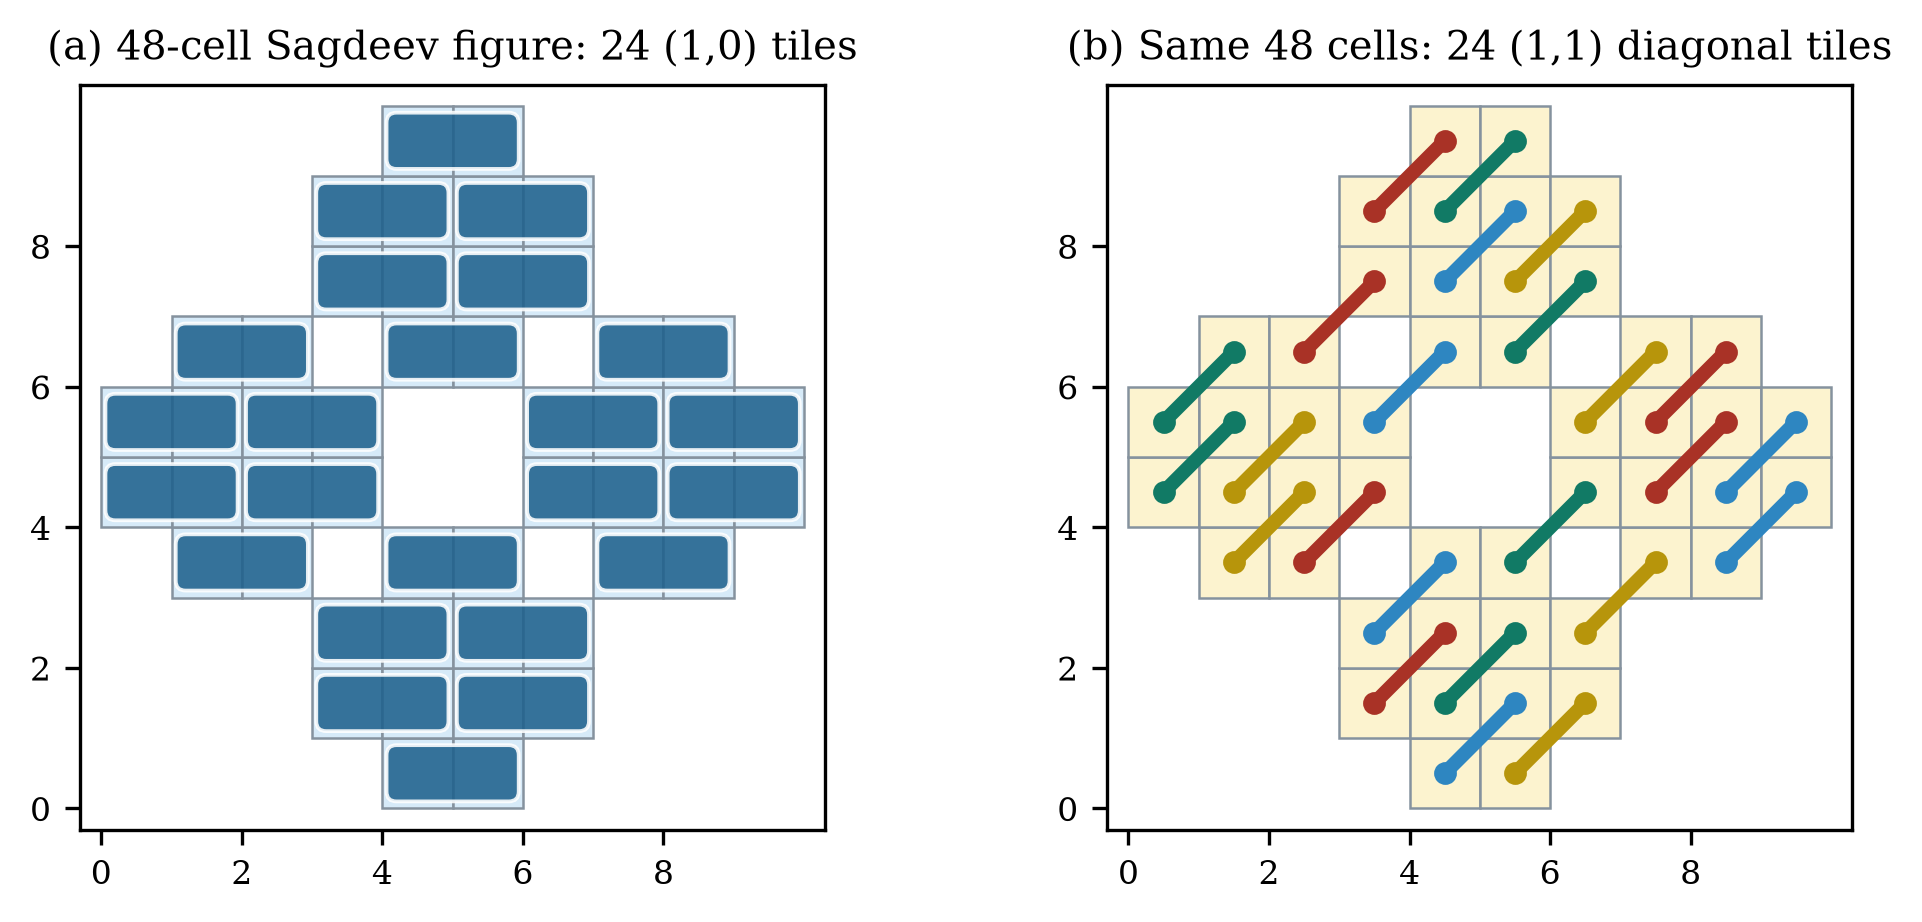
\includegraphics[width=\columnwidth]{figures/fig1_sagdeev_48cell_figure.png}
\caption{Exact $D_4$-symmetric 48-cell 4-direction Sagdeev queen-domino figure: (a)~24 disjoint $(1,0)$ tiles; (b)~24 disjoint $(1,1)$ diagonal tiles (vertical and anti-diagonal tilings follow by $D_4$ symmetry and are independently audited).}
\label{fig:sagdeev}
\end{figure}

\paragraph{2. Quantifying the Step~5--6 gap and Section~2.1 lifts.}
Figure~\ref{fig:gap-boost}(a) exhaustively counts 1D $D_d$-divisible versus $\{0,1\}$-tileable subsets across box lengths $L \in \{4,6,8,10\}$ ($d=2$) and $L \in \{6,9,12\}$ ($d=3$): the strict gap fraction grows rapidly with~$L$, reaching $163/251$ ($64.9\%$) at $d=2, L=10$ and $286/345$ ($82.9\%$) at $d=3, L=12$, demonstrating why Step~6 hole-move repair is essential. Figure~\ref{fig:gap-boost}(b) tracks nonzero Laurent monomials of $f$, $F^*$, and lifted $F$ across our four Section~2.1 divisibility-boosting certificates up to 4 directions ($i=4$).

\begin{figure}[t]
\centering
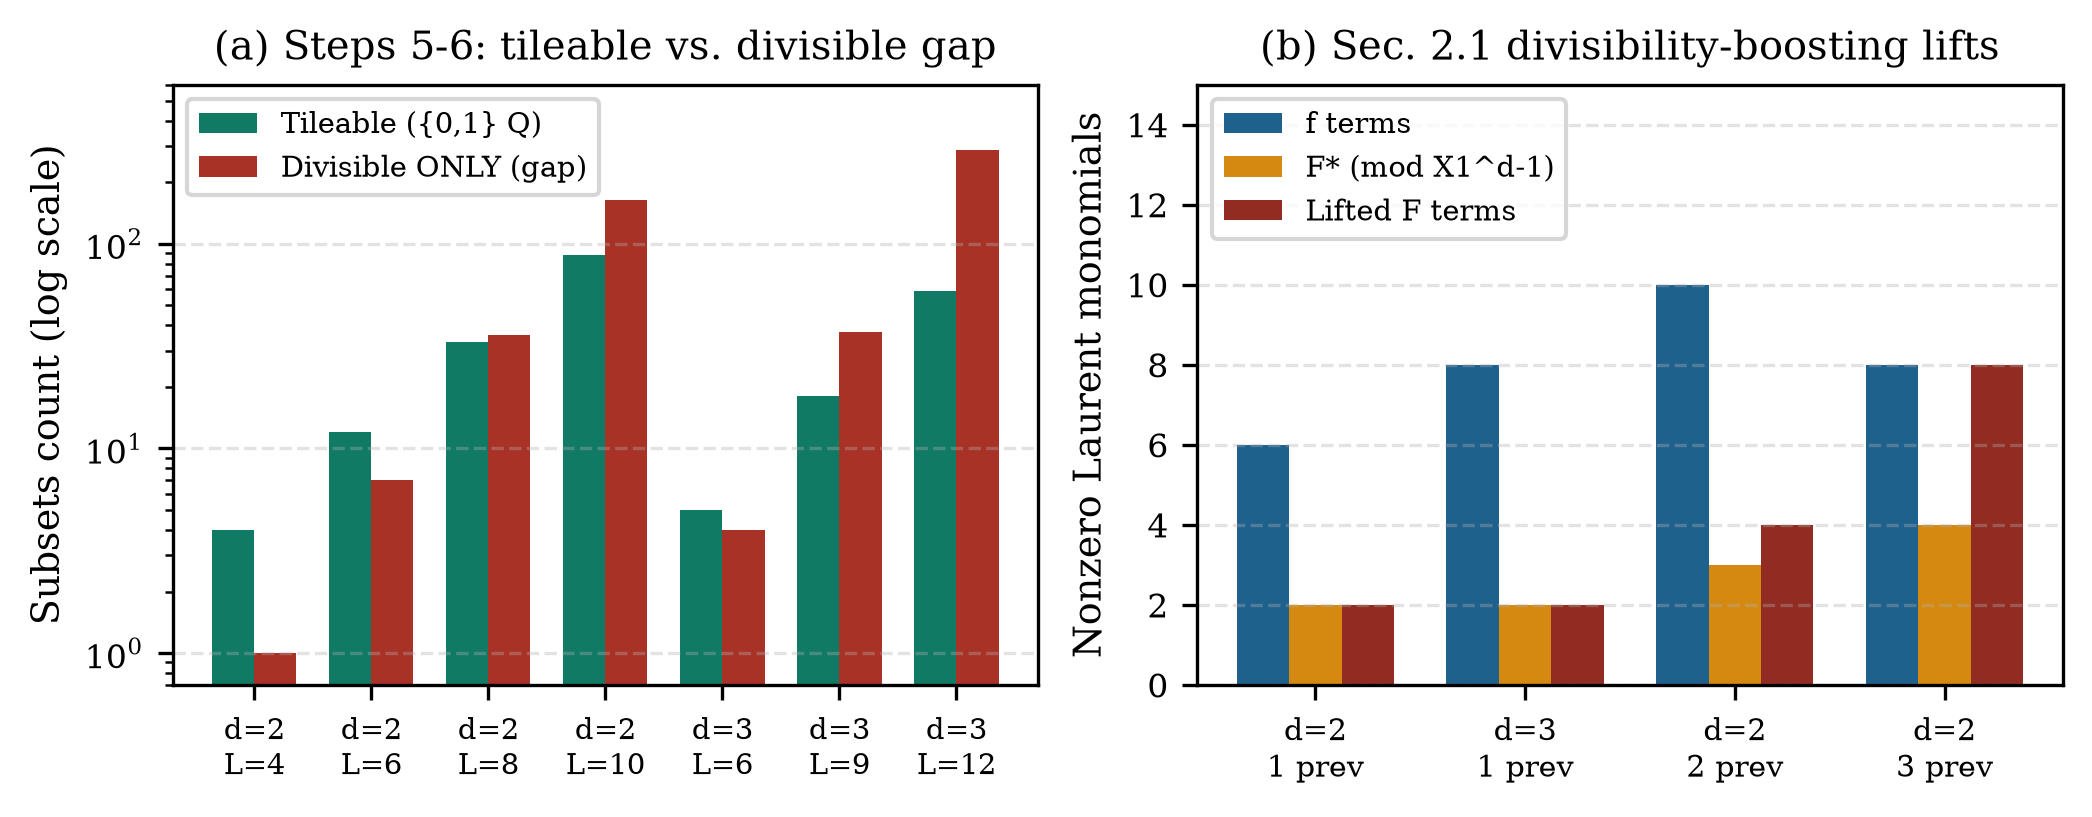
\includegraphics[width=\columnwidth]{figures/fig2_gap_census_and_boosting.png}
\caption{(a)~Exhaustive 1D census of tileable versus strictly tile-divisible-only subsets for $d=2$ ($L=4..10$) and $d=3$ ($L=6..12$). (b)~Monomial support sizes across our four Section~2.1 Laurent divisibility-boosting lifts.}
\label{fig:gap-boost}
\end{figure}

\paragraph{3. 16-certificate atlas and 61-attack red-team suite.}
Table~\ref{tab:atlas} and Figure~\ref{fig:atlas} summarize all 16 canonical certificates, replayed with zero floats in $0.030$--$0.292\,\mathrm{ms}$. In \texttt{tests/test\_suite.py}, independent tests verify the exhaustive $d=2, 3$ gap censuses, confirm exact $D_4$ symmetry and 24-tile counts on the 48-cell Sagdeev figure, replay all 16 certificates, and confirm 61/61 live adversarial forgeries (overlapping tiles, duplicate/sign-reversed APs, non-multiple-$d$ hole moves, already-tileable inputs, $\det(X_1,X_2) \neq 1$, vacuous zero-remainder or unreduced-$F^*$ lifts, broken lift congruences, and wrong LCM counts) are rejected with \texttt{DominoTilingCertificateError}.

\begin{figure}[t]
\centering
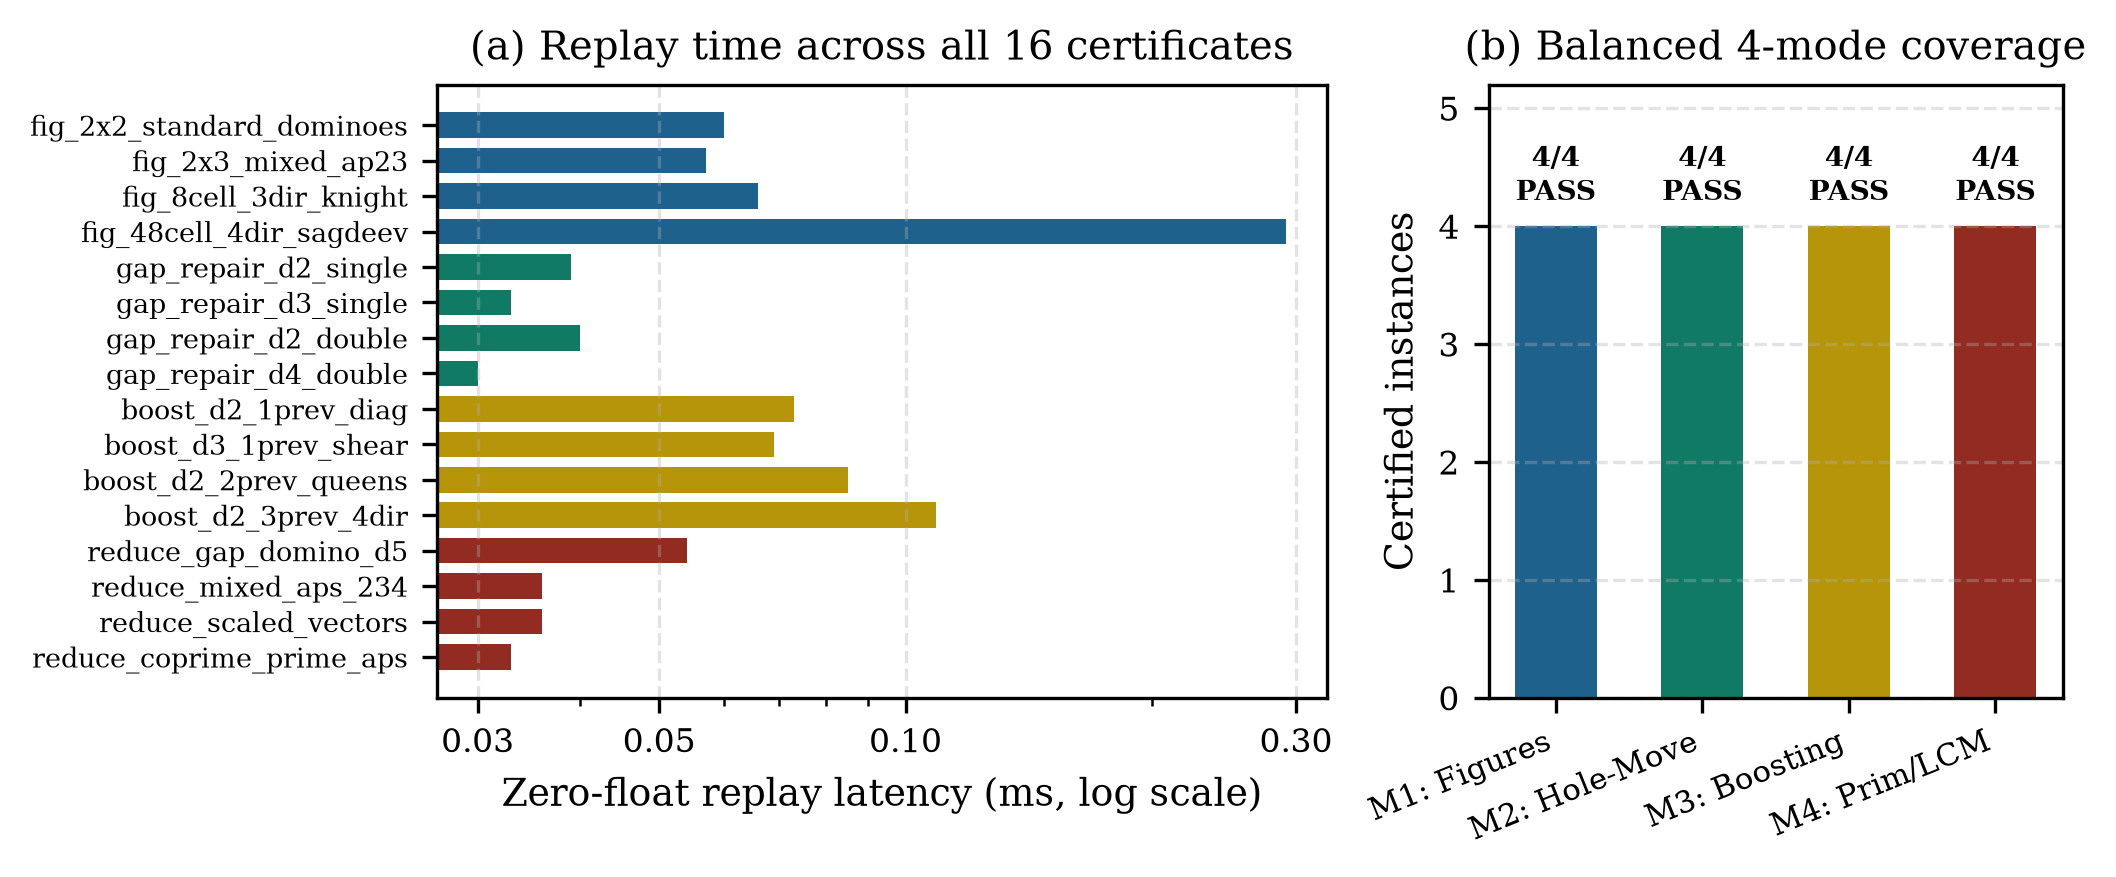
\includegraphics[width=\columnwidth]{figures/fig3_atlas_summary.png}
\caption{(a)~Zero-float replay latency across all 16 canonical \texttt{DOMINO-AP-TILING-CERT-1.0} certificates ($0.030$--$0.292\,\mathrm{ms}$, log scale). (b)~Balanced 4-per-mode coverage across all four verification modes.}
\label{fig:atlas}
\end{figure}

\begin{table}[t]
\centering
\caption{Summary of all 16 exact-$\ZZ$ \texttt{DOMINO-AP-TILING-CERT-1.0} certificates (zero floating-point arithmetic; reference-machine replay latency in ms).}
\label{tab:atlas}
\resizebox{\columnwidth}{!}{%
\begin{tabular}{@{}lllr@{}}
\toprule
Certificate File (stem) & Mode & Key Exact Witness & ms \\
\midrule
\texttt{fig\_2x2\_standard\_dominoes} & M1 & $4$ cells, 2 dirs, $\mathrm{lcm}=2$ & 0.060 \\
\texttt{fig\_2x3\_mixed\_ap23} & M1 & $6$ cells, $d\in\{2,3\}$, $\mathrm{lcm}=6$ & 0.057 \\
\texttt{fig\_8cell\_3dir\_knight} & M1 & $8$ cells, 3 dirs incl.\ $(2,1)$ & 0.066 \\
\texttt{fig\_48cell\_4dir\_sagdeev} & M1 & $48$ cells, 4 queen dirs ($D_4$) & 0.292 \\
\texttt{gap\_repair\_d2\_single} & M2 & $d=2$: $\min Q: -1 \to 0$ (1 move) & 0.039 \\
\texttt{gap\_repair\_d3\_single} & M2 & $d=3$: $\min Q: -1 \to 1$ (1 move) & 0.033 \\
\texttt{gap\_repair\_d2\_double} & M2 & $d=2$: $\min Q: -2 \to 0$ (2 moves) & 0.040 \\
\texttt{gap\_repair\_d4\_double} & M2 & $d=4$: $\min Q: -1 \to 1$ (1 move) & 0.030 \\
\texttt{boost\_d2\_1prev\_diag} & M3 & $d=2$, 1 prev dir, $|f{-}F|_1=8$ & 0.073 \\
\texttt{boost\_d3\_1prev\_shear} & M3 & $d=3$, 1 prev dir, $|f{-}F|_1=8$ & 0.069 \\
\texttt{boost\_d2\_2prev\_queens} & M3 & $d=2$, 2 prev dirs, $|f{-}F|_1=6$ & 0.085 \\
\texttt{boost\_d2\_3prev\_4dir} & M3 & $d=2$, 3 prev dirs, $|f{-}F|_1=8$ & 0.109 \\
\texttt{reduce\_gap\_domino\_d5} & M4 & 5 APs (incl.\ $D_5$), $L=4$ & 0.054 \\
\texttt{reduce\_mixed\_aps\_234} & M4 & $d\in\{2,3,4\} \to L=12$ & 0.036 \\
\texttt{reduce\_scaled\_vectors} & M4 & non-prim $(2,2),(3,0),(0,-2) \to 12$ & 0.036 \\
\texttt{reduce\_coprime\_prime\_aps} & M4 & $d\in\{2,3,5\} \to L=30$ & 0.033 \\
\bottomrule
\end{tabular}}
\end{table}

\section{Scope, Limitations, and Conclusion}\label{sec:conclusion}
This work machine-checks the finite tiling, preprocessing, tile-divisibility gap, step-$d$ hole-move repair, unimodular basis-change, and Laurent divisibility-boosting core of Keevash and Lim~\cite{keevash2026dominoes}, providing a zero-float exact-$\ZZ$ certificate auditor and an explicit 48-cell $D_4$-symmetric 4-direction Sagdeev figure. It does \emph{not} formalize the probabilistic Markov-chain jagged boundary construction, hypergraph almost-perfect matching nibble, or general existence proof of Theorem~1.2 in Lean~4. Within its verified scope, the Lean~4 kernel and \texttt{DOMINO-AP-TILING-CERT-1.0} auditor deliver exact, manifest-locked verification for simultaneous lattice AP tilings and absorption lifts.

\bibliographystyle{plain}
\bibliography{references}
\end{document}
